\begin{figure*}
    \centering
    \begin{subfigure}[t]{0.31\textwidth}
        \vspace{0px}
        \centering
        \begin{subfigure}[t]{0.475\textwidth}
            \vspace{0px}
            \centering
            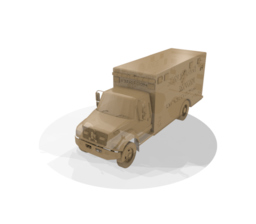
\includegraphics[width=2.5cm,trim={0.25cm 0.5cm 1.5cm 1.5cm},clip]{gfx/appendix_experiments_shapenet/meshes/00014}
        \end{subfigure}
        \begin{subfigure}[t]{0.475\textwidth}
            \vspace{0px}
            \centering
            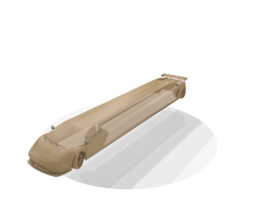
\includegraphics[width=2.5cm,trim={0.25cm 0.5cm 1.5cm 1.5cm},clip]{gfx/appendix_experiments_shapenet/meshes/00007}
        \end{subfigure}\\
        \begin{subfigure}[t]{0.475\textwidth}
            \vspace{0px}
            \centering
            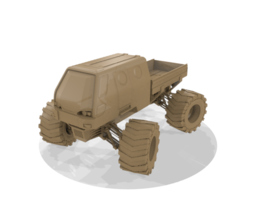
\includegraphics[width=2.5cm,trim={0.25cm 0.5cm 1.5cm 1.5cm},clip]{gfx/appendix_experiments_shapenet/meshes/00017}
        \end{subfigure}
        \begin{subfigure}[t]{0.475\textwidth}
            \vspace{0px}
            \centering
            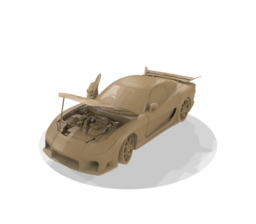
\includegraphics[width=2.5cm,trim={0.25cm 0.5cm 1.5cm 1.5cm},clip]{gfx/appendix_experiments_shapenet/meshes/00013}
        \end{subfigure}
    \end{subfigure} 
    {\color{black!25}\vrule width 0.5px}
    \begin{subfigure}[t]{0.31\textwidth}
        \vspace{0px}
        \centering
        \begin{subfigure}[t]{0.475\textwidth}
            \vspace{0px}
            \centering
            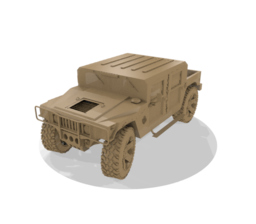
\includegraphics[width=2.5cm,trim={0.25cm 0.5cm 1.5cm 1.5cm},clip]{gfx/appendix_experiments_shapenet/meshes/00000}
        \end{subfigure}
        \begin{subfigure}[t]{0.475\textwidth}
            \vspace{0px}
            \centering
            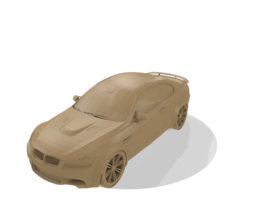
\includegraphics[width=2.5cm,trim={0.25cm 0.5cm 1.5cm 1.5cm},clip]{gfx/appendix_experiments_shapenet/meshes/00002}
        \end{subfigure}\\
        \begin{subfigure}[t]{0.475\textwidth}
            \vspace{0px}
            \centering
            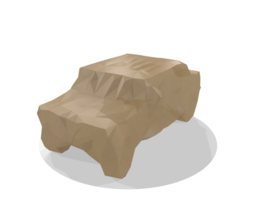
\includegraphics[width=2.5cm,trim={0.25cm 0.5cm 1.5cm 1.5cm},clip]{gfx/appendix_experiments_shapenet/meshes/00001}
        \end{subfigure}
        \begin{subfigure}[t]{0.475\textwidth}
            \vspace{0px}
            \centering
            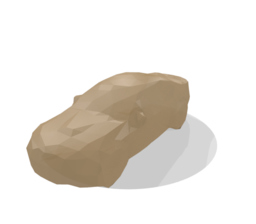
\includegraphics[width=2.5cm,trim={0.25cm 0.5cm 1.5cm 1.5cm},clip]{gfx/appendix_experiments_shapenet/meshes/00003}
        \end{subfigure}
    \end{subfigure}
    {\color{black!25}\vrule width 0.5px}
    \begin{subfigure}[t]{0.31\textwidth}
        \vspace{0px}
        \centering
        \begin{subfigure}[t]{0.475\textwidth}
            \vspace{0px}
            \centering
            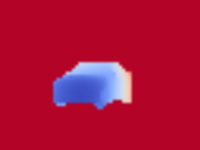
\includegraphics[width=2.5cm]{gfx/appendix_experiments_shapenet/depths/18}
        \end{subfigure}
        \begin{subfigure}[t]{0.475\textwidth}
            \vspace{0px}
            \centering
            
\includegraphics[width=2.5cm]{gfx/appendix_experiments_shapenet/depths/54}
        \end{subfigure}\\[0.15cm]
        \begin{subfigure}[t]{0.475\textwidth}
            \vspace{0px}
            \centering
            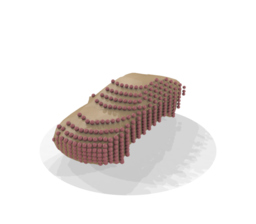
\includegraphics[width=2.5cm,trim={0.25cm 0.5cm 1.5cm 1.5cm},clip]{gfx/experiments_data/clean*/simplified/00001}
        \end{subfigure}
        \begin{subfigure}[t]{0.475\textwidth}
            \vspace{0px}
            \centering
            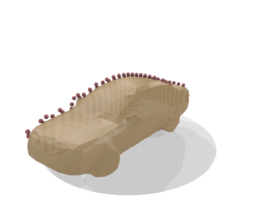
\includegraphics[width=2.5cm,trim={0.25cm 0.5cm 1.5cm 1.5cm},clip]{gfx/experiments_data/clean*/simplified/00009}
        \end{subfigure}
    \end{subfigure}
    \caption{{\bf Left: Examples of Discarded ShapeNet Models.} We manually discarded 262 of ShapeNet's \cite{Chang2015ARXIV} car models by inspecting top-views of the corresponding meshes. Most of the discarded models represent large, elongated or exotic cars such as trucks, limousines or monster trucks. Other models also include opened doors or other unwanted settings. {\bf Middle: Simplification Examples.} The used simplification algorithm \cite{Guney2015CVPR} reduces all models to exactly $1k$ faces; for some models this results in crude approximations, for others, only minor details are lost. We show the original models (top) and the corresponding simplified models (bottom). {\bf Right: Rendering Examples.} Illustration of our rendering process for \clean where a model is rendered into a depth image from a random viewpoint around the car. We show the rendered depth image (top; {\color{red}red} is background, {\color{blue}blue} is closer) and the corresponding model (bottom; {\color{rbeige}beige}) including observations (bottom; {\color{rred}red}).}
    \label{fig:appendix-experiments-shapenet}
\end{figure*}